\documentclass[10.5pt,a4paper]{ctexart}
\usepackage[margin=1.75cm,headheight=14pt]{geometry}
\usepackage{graphicx,booktabs,tabularx,array,float,xcolor,amsmath,amssymb,fancyhdr,hyperref,caption}
\usepackage{enumitem,titlesec}
\definecolor{navy}{HTML}{2F5597}\definecolor{green}{HTML}{548235}\definecolor{light}{HTML}{EAF0F8}
\hypersetup{colorlinks=true,linkcolor=navy,urlcolor=navy}
\captionsetup{font=small,labelfont=bf,skip=3pt}
\setlength{\parindent}{2em}\setlength{\parskip}{0.12em}
\setlength{\textfloatsep}{7pt plus 2pt minus 2pt}
\setlength{\floatsep}{6pt plus 2pt minus 2pt}
\setlength{\intextsep}{6pt plus 2pt minus 2pt}
\titlespacing*{\section}{0pt}{1.1ex plus .3ex}{0.55ex}
\titlespacing*{\subsection}{0pt}{0.8ex plus .2ex}{0.35ex}
\setlist[itemize]{nosep,leftmargin=1.7em}
\pagestyle{fancy}\fancyhf{}\lhead{CF2026 Project 1}\rhead{A股多因子研究平台}\cfoot{\thepage}
\newcommand{\key}[1]{\textcolor{navy}{\textbf{#1}}}
\newcommand{\code}[1]{\texttt{\small #1}}
\begin{document}

\begin{titlepage}
\centering
\vspace*{2.0cm}
{\Huge\bfseries A股多因子选股与风险控制研究\par}
\vspace{0.6cm}
{\Large 按数据、信号、组合、成交、净值与评价顺序构建研究闭环\par}
\vspace{1.6cm}
\begin{minipage}{0.88\textwidth}
\textbf{摘要}\quad 本文按照“数据--因子/信号--目标组合--回测/模拟成交--策略净值--评价与解释”的顺序，搭建一个完整、正确、可复现且可扩展的量化研究平台。基础研究在动态沪深主板资产池中，从7个候选因子选择20日低波动、5日反转和20日Amihud非流动性，形成Top 20等权组合，并在停牌、涨跌停、退市与交易费用约束下逐日模拟成交。对照实验仅改变调仓频率，结果显示月频相较周频具有更低换手和成本，并取得28.34\%年化收益、1.214 Sharpe和30.04\%最大回撤。拓展实验另行比较波动率目标、ERC风险平价、权重上限、动态沪深300机器学习和研究工作台；其中15\%波动率目标在收益保留与风险下降之间较均衡。机器学习结果作为附加探索报告，不改变基础研究结论。

\vspace{0.7cm}
\textbf{关键词：}A股；多因子；动态资产池；Rank IC；模拟成交；交易成本；风险控制
\end{minipage}
\vfill
{\large 计算金融 Project 1\par}
\vspace{0.4cm}
{\large 报告生成日期：2026年9月\par}
\end{titlepage}

\section{研究问题与系统框架}
\subsection{研究目标}
本项目的目标不是寻找样本内收益最高的参数，而是建立一个\key{完整、正确、可复现、可扩展}的研究平台。主线问题是：三个经济逻辑不同的因子能否在交易限制和费用下形成可执行组合；在保持其他条件不变时，降低调仓频率能否改善成本、回撤与稳定性。风险控制和机器学习均作为主线完成后的拓展实验。

\begin{figure}[H]\centering
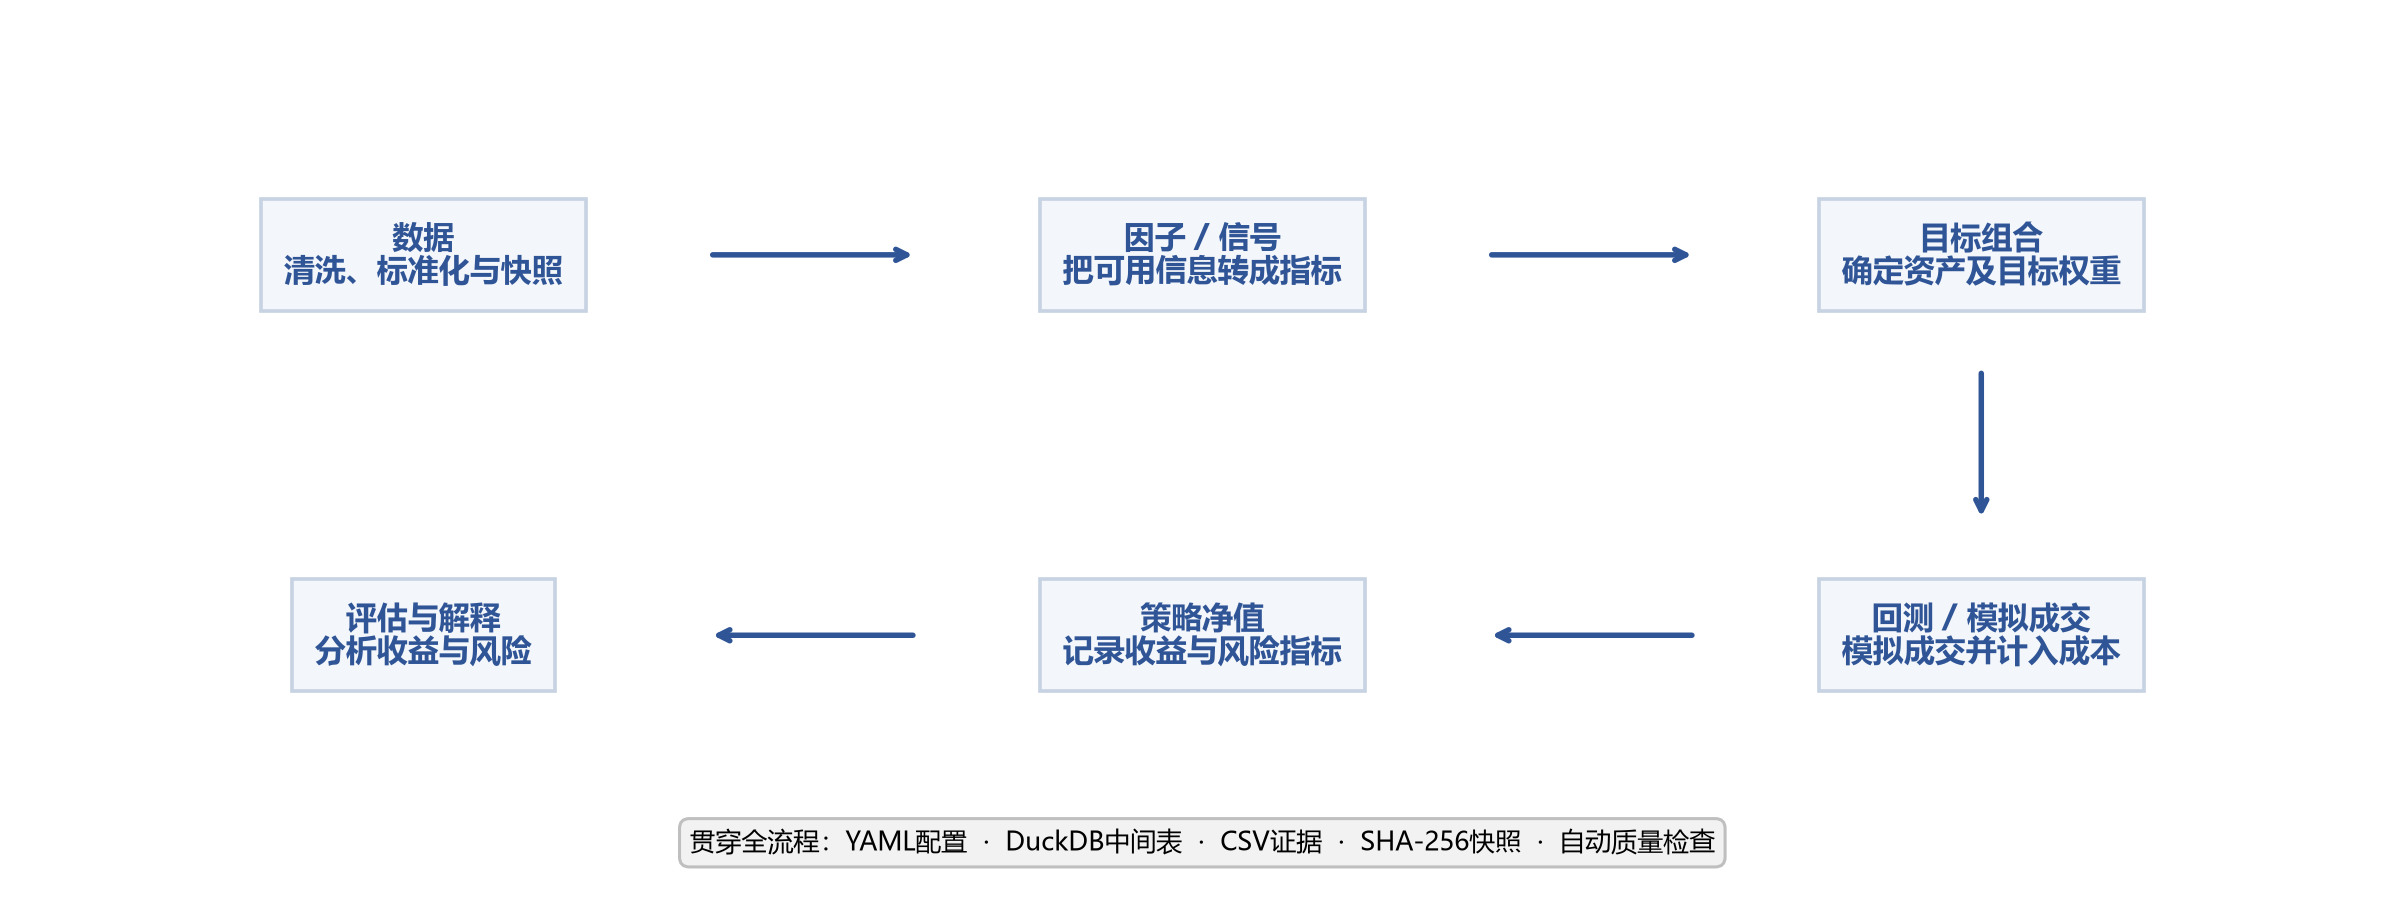
\includegraphics[width=\textwidth]{figures/01_research_architecture.png}
\caption{研究框架与模块连接关系}
\end{figure}

系统将数据、因子、目标组合、成交模拟和绩效分析分离。因子模块只输出统一长表，回测模块只读取信号和配置；替换因子或组合规则时无需改写成交核心。关键中间表保存于DuckDB，证据输出为CSV，并使用SHA-256冻结数据、代码与结果版本。

\subsection{研究步骤}
全文严格按照平台的数据流顺序展开：
\begin{enumerate}[nosep,leftmargin=2.2em]
\item \textbf{数据：}确定研究范围，下载并冻结原始快照，完成复权、清洗和动态资产池；
\item \textbf{因子/信号：}定义候选因子，统一方向与缺失规则，并用IC、Rank IC和五分组诊断；
\item \textbf{目标组合：}选择三个逻辑不同的因子，形成Top 20等权目标；
\item \textbf{回测/模拟成交：}以前一交易日信号在下一交易日开盘成交，处理现金、停牌、涨跌停、退市与费用；
\item \textbf{策略净值：}逐日记录持仓、交易、成本、收益和净值并完成对账；
\item \textbf{评价与解释：}报告收益、波动、Sharpe、回撤、换手和成本，再分别开展对照实验与拓展实验。
\end{enumerate}

\subsection{研究边界}
基础实验研究上交所和深交所主板A股。本文未把收益率达标作为模型正确性的标准，而是优先检查唯一键、未来信息、费用对账、资产池变化和重复运行一致性。动态沪深300及模型实验只在拓展章节出现。

\subsection{主要结果概览}
主线结果是：从7个候选因子中选出低波动、短期反转与Amihud非流动性；月频三因子组合年化收益28.34\%，相较周频显著降低换手与显式成本。拓展实验中，15\%波动率目标把年化波动降至17.99\%、最大回撤降至25.21\%，同时保留24.23\%年化收益。机器学习与网页工作台单独列为附加拓展，不与基础策略混为同一个结论。

\section{数据、样本与清洗}
\subsection{数据范围与价格口径}
数据来自Tushare Pro。正式研究期为2020-01-01至2025-12-31，下载缓冲期为2019-10-01至2026-01-31，用于滚动窗口和未来收益标签。日线成交量单位为手（1手=100股），成交额单位为千元。原始价、复权因子及复权价分别保存，开盘与收盘采用同一参考因子：
\[
P^{adj}_{i,t}=P^{raw}_{i,t}\frac{a_{i,t}}{a_{i,\tau}},
\]
其中$a_{i,t}$为复权因子，$\tau$为固定参考日。该口径避免把不同参考日的价格片段直接拼接。

\begin{table}[H]\centering\small
\caption{正式下载并导入数据库的数据规模}
\begin{tabular}{lrrl}
\toprule 数据集 & 记录数 & 主要用途 & 保存口径\\\midrule
日线行情 & 7,433,025 & 价格、收益、成交量与成交额 & 原始层\\
复权因子 & 7,579,193 & 统一开盘和收盘复权口径 & 原始层\\
股票基础信息 & 5,904 & 交易所、板块、上市与退市日期 & 参考层\\
交易日历 & 2,315 & 日期合法性和调仓日 & 参考层\\
历史名称 & 10,763 & 构造逐日历史ST状态 & 参考层\\
停牌记录 & 57,786 & 限制不可成交日期 & 约束层\\
涨跌停价格 & 7,482,828 & 判断开盘涨跌停 & 约束层\\\bottomrule
\end{tabular}
\end{table}

\subsection{动态资产池与清洗规则}
每个交易日依据股票代码、上市/退市日期、交易所、板块和历史名称判断是否入池。历史名称区间含ST标识的日期被排除；停牌记录不从资产定义中永久删除，而由成交层决定当日不可交易。每行由\code{trade\_date + ts\_code}唯一标识。缺失值不统一填零，成交量为零保留并单独标记。

\begin{table}[H]\centering\small
\caption{7,433,025条日线行情的互斥清洗对账}
\begin{tabular}{lrrp{6.2cm}}
\toprule 处理结果 & 记录数 & 占输入比例 & 原因与处理\\\midrule
缺少股票元数据 & 1,337 & 0.018\% & 无法可靠判断交易所、板块或上市区间，排除并记录\\
不属于动态研究资产池 & 2,663,175 & 35.829\% & 非沪深主板或不在当日上市区间，不进入研究样本\\
历史ST日期 & 202,719 & 2.727\% & 名称生效区间显示ST/退市风险警示，按研究定义排除\\
最终保留记录 & 4,565,794 & 61.426\% & 满足元数据、上市区间、市场范围与非ST要求\\\midrule
对账总数 & 7,433,025 & 100.000\% & 四类互斥，清洗前后数量完全对应\\\bottomrule
\end{tabular}
\end{table}

\begin{table}[H]\centering\small
\caption{清洗后的可验证质量提升}
\begin{tabular}{lrrl}
\toprule 质量问题 & 输入层识别数 & 清洗表剩余数 & 改善结果\\\midrule
缺少股票元数据 & 1,337 & 0 & 保留记录均可识别资产身份与市场\\
资产池外记录 & 2,663,175 & 0 & 保留记录均符合逐日沪深主板定义\\
历史ST记录 & 202,719 & 0 & 研究样本与非ST口径一致\\
重复日期--资产键 & 检查 & 0 & 每只股票每日最多一条记录\\
非法价格、成交量或关键标识 & 检查 & 0 & 后续收益与成交计算无非法输入\\\bottomrule
\end{tabular}
\end{table}

清洗并非简单追求保留率，而是把无法定义、超出研究范围或与非ST假设冲突的记录显式隔离。动态资产池范围内，在排除历史ST之前共有4,768,513条候选记录，最终保留其中95.75\%。停牌417条、开盘涨停14,712条和开盘跌停8,298条没有被静默删除，而是保留状态标记并交给回测执行层处理。原始层与清洗层分开保存，9,503个原始文件均记录大小与SHA-256。

\section{因子设计与预处理}
\subsection{候选因子及经济逻辑}
\begin{table}[H]\centering\small
\caption{七个候选因子}
\begin{tabularx}{\textwidth}{lllX}
\toprule 因子 & 类型 & 方向 & 研究假设\\\midrule
20日动量 & 动量 & 正 & 中短期趋势可能延续\\
5日反转 & 反转 & 负近期收益 & 短期过度反应可能修复\\
20日低波动 & 风险 & 负波动 & 低风险股票可能更稳定\\
60日跳过5日动量 & 动量 & 正 & 中期趋势并规避短期反转\\
5日隔夜反转 & 反转 & 负隔夜收益 & 隔夜过度反应可能在日内修复\\
20日Amihud非流动性 & 流动性 & 正 & 价格冲击可能对应流动性溢价\\
5/20日成交活跃度变化 & 成交量 & 正 & 放量可能表示新信息进入市场\\
\bottomrule
\end{tabularx}
\end{table}

每个因子均有因子卡，记录研究假设、公式、字段、窗口、预期方向、缺失规则和可能失效情形。统一输出为\code{date, asset, factor, value}。历史不足时记缺失，不填零。

\begin{table}[H]\centering\scriptsize
\caption{七张因子卡：定义、数据字段与窗口}
\begin{tabularx}{\textwidth}{p{2.2cm}p{2.5cm}Xp{2.1cm}p{2.5cm}}
\toprule 名称 & 研究假设 & 公式 & 字段 & 窗口\\\midrule
20日动量 & 中短期强势可能延续 & $C_t/C_{t-20}-1$ & 复权收盘价 & 20个连续交易日\\
5日反转 & 短期过度反应可能修复 & $-(C_t/C_{t-5}-1)$ & 复权收盘价 & 5个连续交易日\\
20日低波动 & 低波动股票可能更稳定 & $-std(r,20)$ & 复权收盘价 & 20个日收益\\
60日跳过5日动量 & 中期趋势延续并避开短期反转 & $C_{t-5}/C_{t-60}-1$ & 复权收盘价 & 60日，跳过最近5日\\
5日隔夜反转 & 隔夜涨幅过大可能回调 & $-\sum_{5}\log(O_t/C_{t-1})$ & 复权开盘、收盘 & 5个有效隔夜\\
20日Amihud非流动性 & 非流动性可能要求收益补偿 & $\log(mean(|r|/Amount,20))$ & 收盘价、成交额 & 20个连续交易日\\
5/20日成交活跃度变化 & 放量可能表示新信息进入 & $\log(\bar A_5/\bar A_{20})$ & 成交额 & 5日与20日\\\bottomrule
\end{tabularx}
\end{table}

\begin{table}[H]\centering\scriptsize
\caption{七张因子卡：方向、缺失处理与可能失效情形}
\begin{tabularx}{\textwidth}{p{2.3cm}p{2.1cm}Xp{4.0cm}}
\toprule 名称 & 统一方向 & 缺失处理 & 可能失效情形\\\midrule
20日动量 & 越高越好 & 历史不足20日或窗口含无效行情则缺失 & 趋势快速反转或动量崩溃\\
5日反转 & 取负后越高越好 & 历史不足5日或窗口不连续则缺失 & 强趋势行情\\
20日低波动 & 波动率取负 & 有效日收益不足20个则缺失 & 高风险偏好或急涨行情\\
60日跳过5日动量 & 越高越好 & 60日窗口不完整则缺失 & 趋势切换或行情反转\\
5日隔夜反转 & 隔夜收益取负 & 停牌、ST或非连续交易日不跨越计算 & 持续信息驱动的跳空趋势\\
20日Amihud非流动性 & 越高越非流动 & 收益缺失或成交额非正则缺失 & 成本吞噬溢价或小盘股混杂\\
5/20日成交活跃度变化 & 越高越放量 & 20日窗口不完整或成交额非正则缺失 & 投机放量后反转\\\bottomrule
\end{tabularx}
\end{table}

\subsection{截面预处理}
因子公式与回测核心分离：\code{factor\_cards.yaml}保存说明书，\code{factor\_config.yaml}控制启用因子、窗口与预处理，计算模块统一输出长表。每条记录为：
\begin{center}\small
\begin{tabular}{llll}\toprule date & asset & factor & value\\\midrule
2025-01-02 & 000001.SZ & low\_volatility\_20 & $-0.0126$\\
2025-01-02 & 000002.SZ & reversal\_5 & $0.0314$\\\bottomrule\end{tabular}
\end{center}
每日截面依次保留原始值、按1\%/99\%分位缩尾、计算Z-score并生成百分位排名。缩尾防止极端异常值支配结果，Z-score用于三个因子等权合成，百分位排名用于分组与相对强弱比较。所有信号统一为“分数越高，预期收益越高”；反转和低波动因子通过取负号完成方向统一。基础版将中性化显式配置为关闭，因此可能保留行业或规模暴露，并在局限中说明。

\subsection{逻辑差异}
因子差异同时从经济机制、Rank相关性和高分组重合率判断。最终三个因子分别代表风险、短期价格行为和流动性，不仅名称不同，其数据变换与可能失效机制也不同。

\section{因子诊断与选择}
固定持有期$h$下，在形成日$t$的有效资产集合上计算：
\[
IC_t^{(h)}=Corr(f_{i,t},y_{i,t}^{(h)}),\qquad
RankIC_t^{(h)}=Corr(rank(f_{i,t}),rank(y_{i,t}^{(h)})).
\]
标签从下一交易日开始，构建1、5和20日未来收益。五分组按形成日因子值排序，组内等权；标签缺失不重新分组。分组诊断不连续复利为策略净值。

\begin{figure}[H]\centering
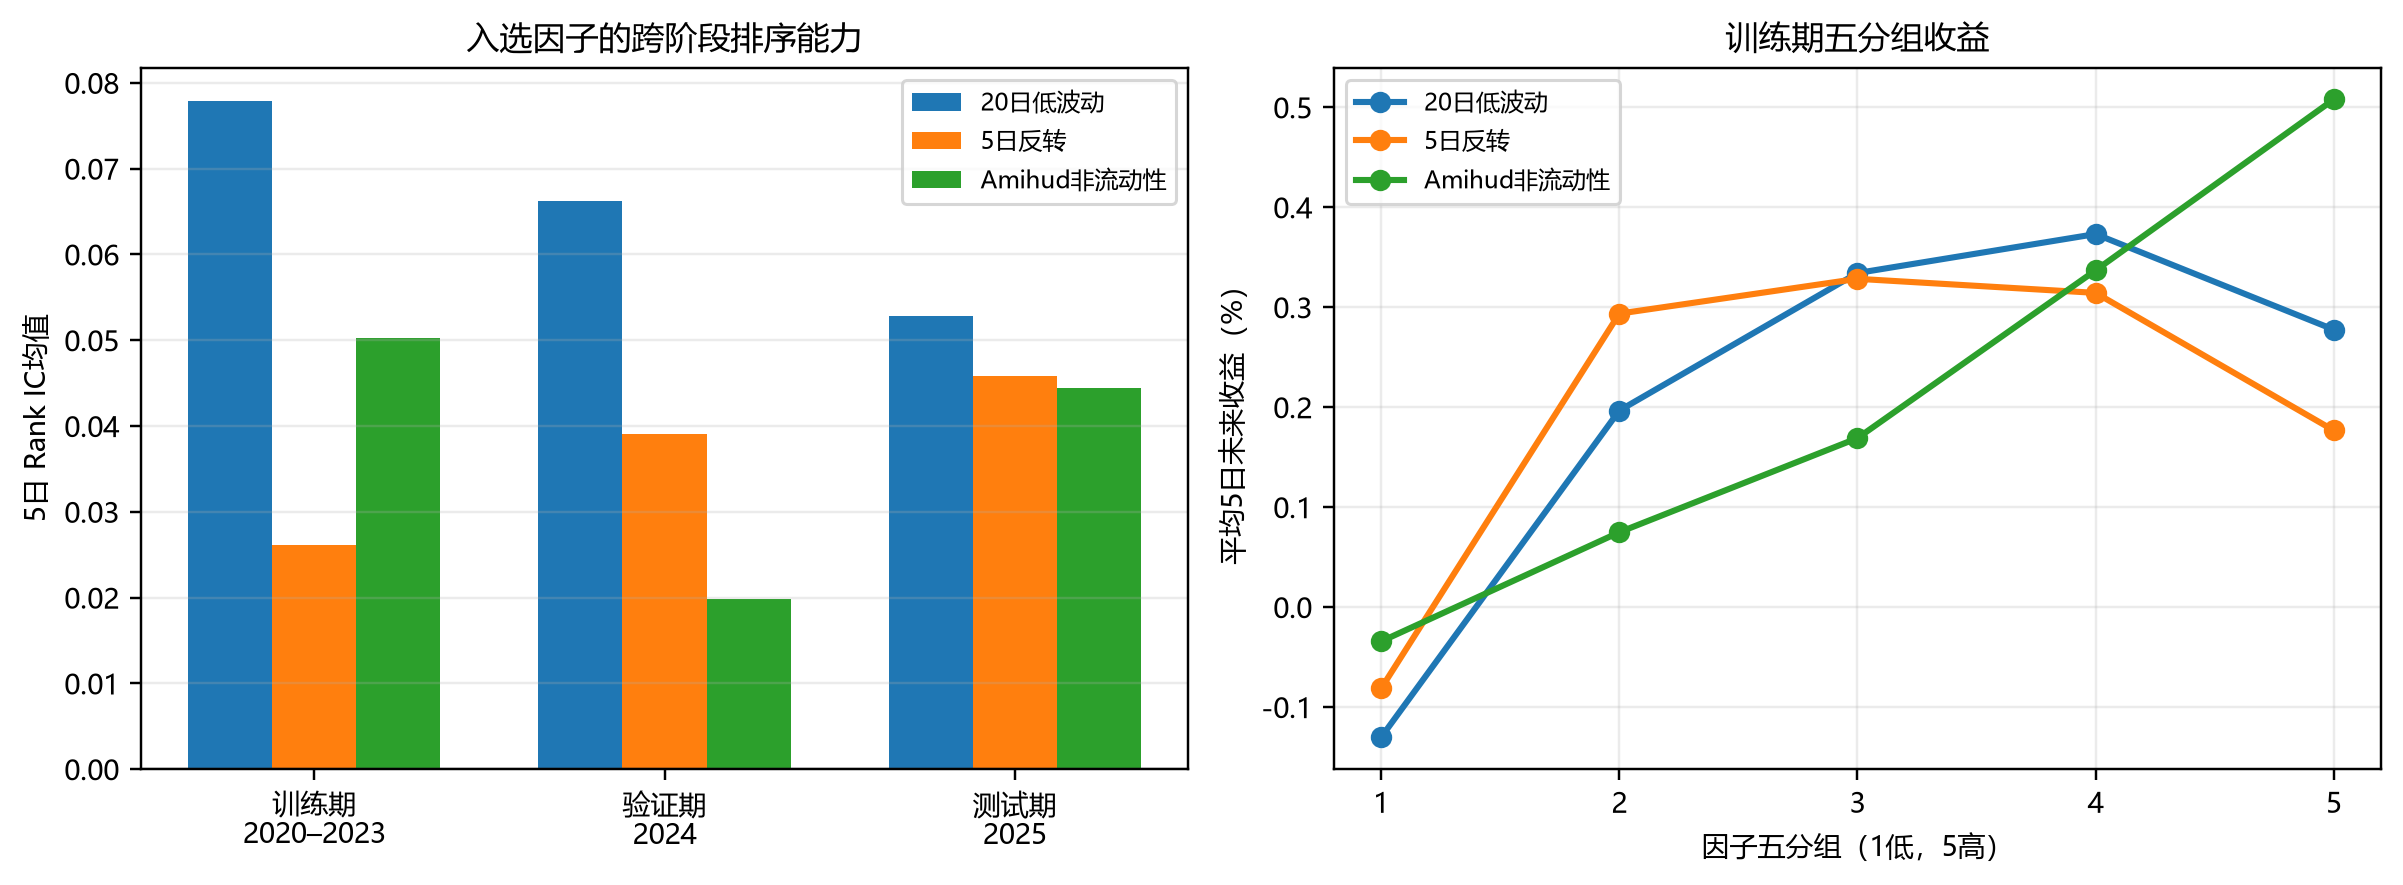
\includegraphics[width=\textwidth]{figures/02_factor_diagnostics.png}
\caption{入选因子的Rank IC与五分组收益诊断}
\end{figure}

因子选择只使用2020--2023训练期和2024验证期，2025作为选择后的测试期报告。综合IC、Rank IC、五分组价差、覆盖率和逻辑差异，选择\key{20日低波动、5日反转和20日Amihud非流动性}。三者Z-score等权平均形成综合信号。

这里的IC和t统计量仅作描述性诊断。多日标签重叠、时间序列相关和多候选因子搜索会影响传统显著性判断，本文不将其解释为严格的因果证据或未来收益保证。

\section{目标组合、模拟成交与策略净值}
\subsection{目标组合}
综合因子每日按截面排名，调仓时选择前20只，基础组合目标等权。目标表只描述希望持有的资产和权重，不假设目标能够立即成交；信号形成日期、目标权重和实际成交结果分别保存。

\subsection{回测与模拟成交}
信号使用调仓日前一交易日收盘后数据，下一交易日开盘成交。开盘涨停不买、开盘跌停不卖、停牌或零成交量不交易，未成交旧仓继续保留。退市后仍无法卖出的持仓按零回收率核销，以避免使用陈旧价格虚增净值。

交易成本为
\[
Cost_t=c_bB_t+c_sS_t,
\]
其中买入费率$c_b=0.03\%$，卖出费率$c_s=0.13\%$，只对实际成交额收费。初始资金为100万元，无风险收益率设为0。回测输出日收益、净值、持仓、交易日志、双边换手和累计费用。

\subsection{策略净值、评价与一致性检查}
报告累计和年化收益、年化波动率、Sharpe、最大回撤、换手、成本、持仓数、最大单股权重及交易次数。净值与日收益独立复核，累计收益误差约$10^{-14}$；每日费用、指标费用和累计费用误差不超过$10^{-8}$容差。目标持仓形成日严格早于调仓日。

基础周频三因子策略年化收益20.40\%、年化波动23.93\%、Sharpe 0.897、最大回撤40.21\%。三个单因子在加入费用、交易限制和退市核销后表现明显弱于组合，说明因子诊断的排序能力不等于单一可交易策略的净收益。

\section{对照实验：周频与月频}
\subsection{实验设计}
对照实验只改变调仓频率：周频使用每周首个交易日，月频使用每月首个交易日。两组共用相同数据快照、2020--2025样本、动态资产池、三因子、Top 20等权目标、费率和成交限制。自动检查确认两组均覆盖1,455个交易日，无未来信息；周频307次调仓，月频71次调仓。

\begin{figure}[H]\centering
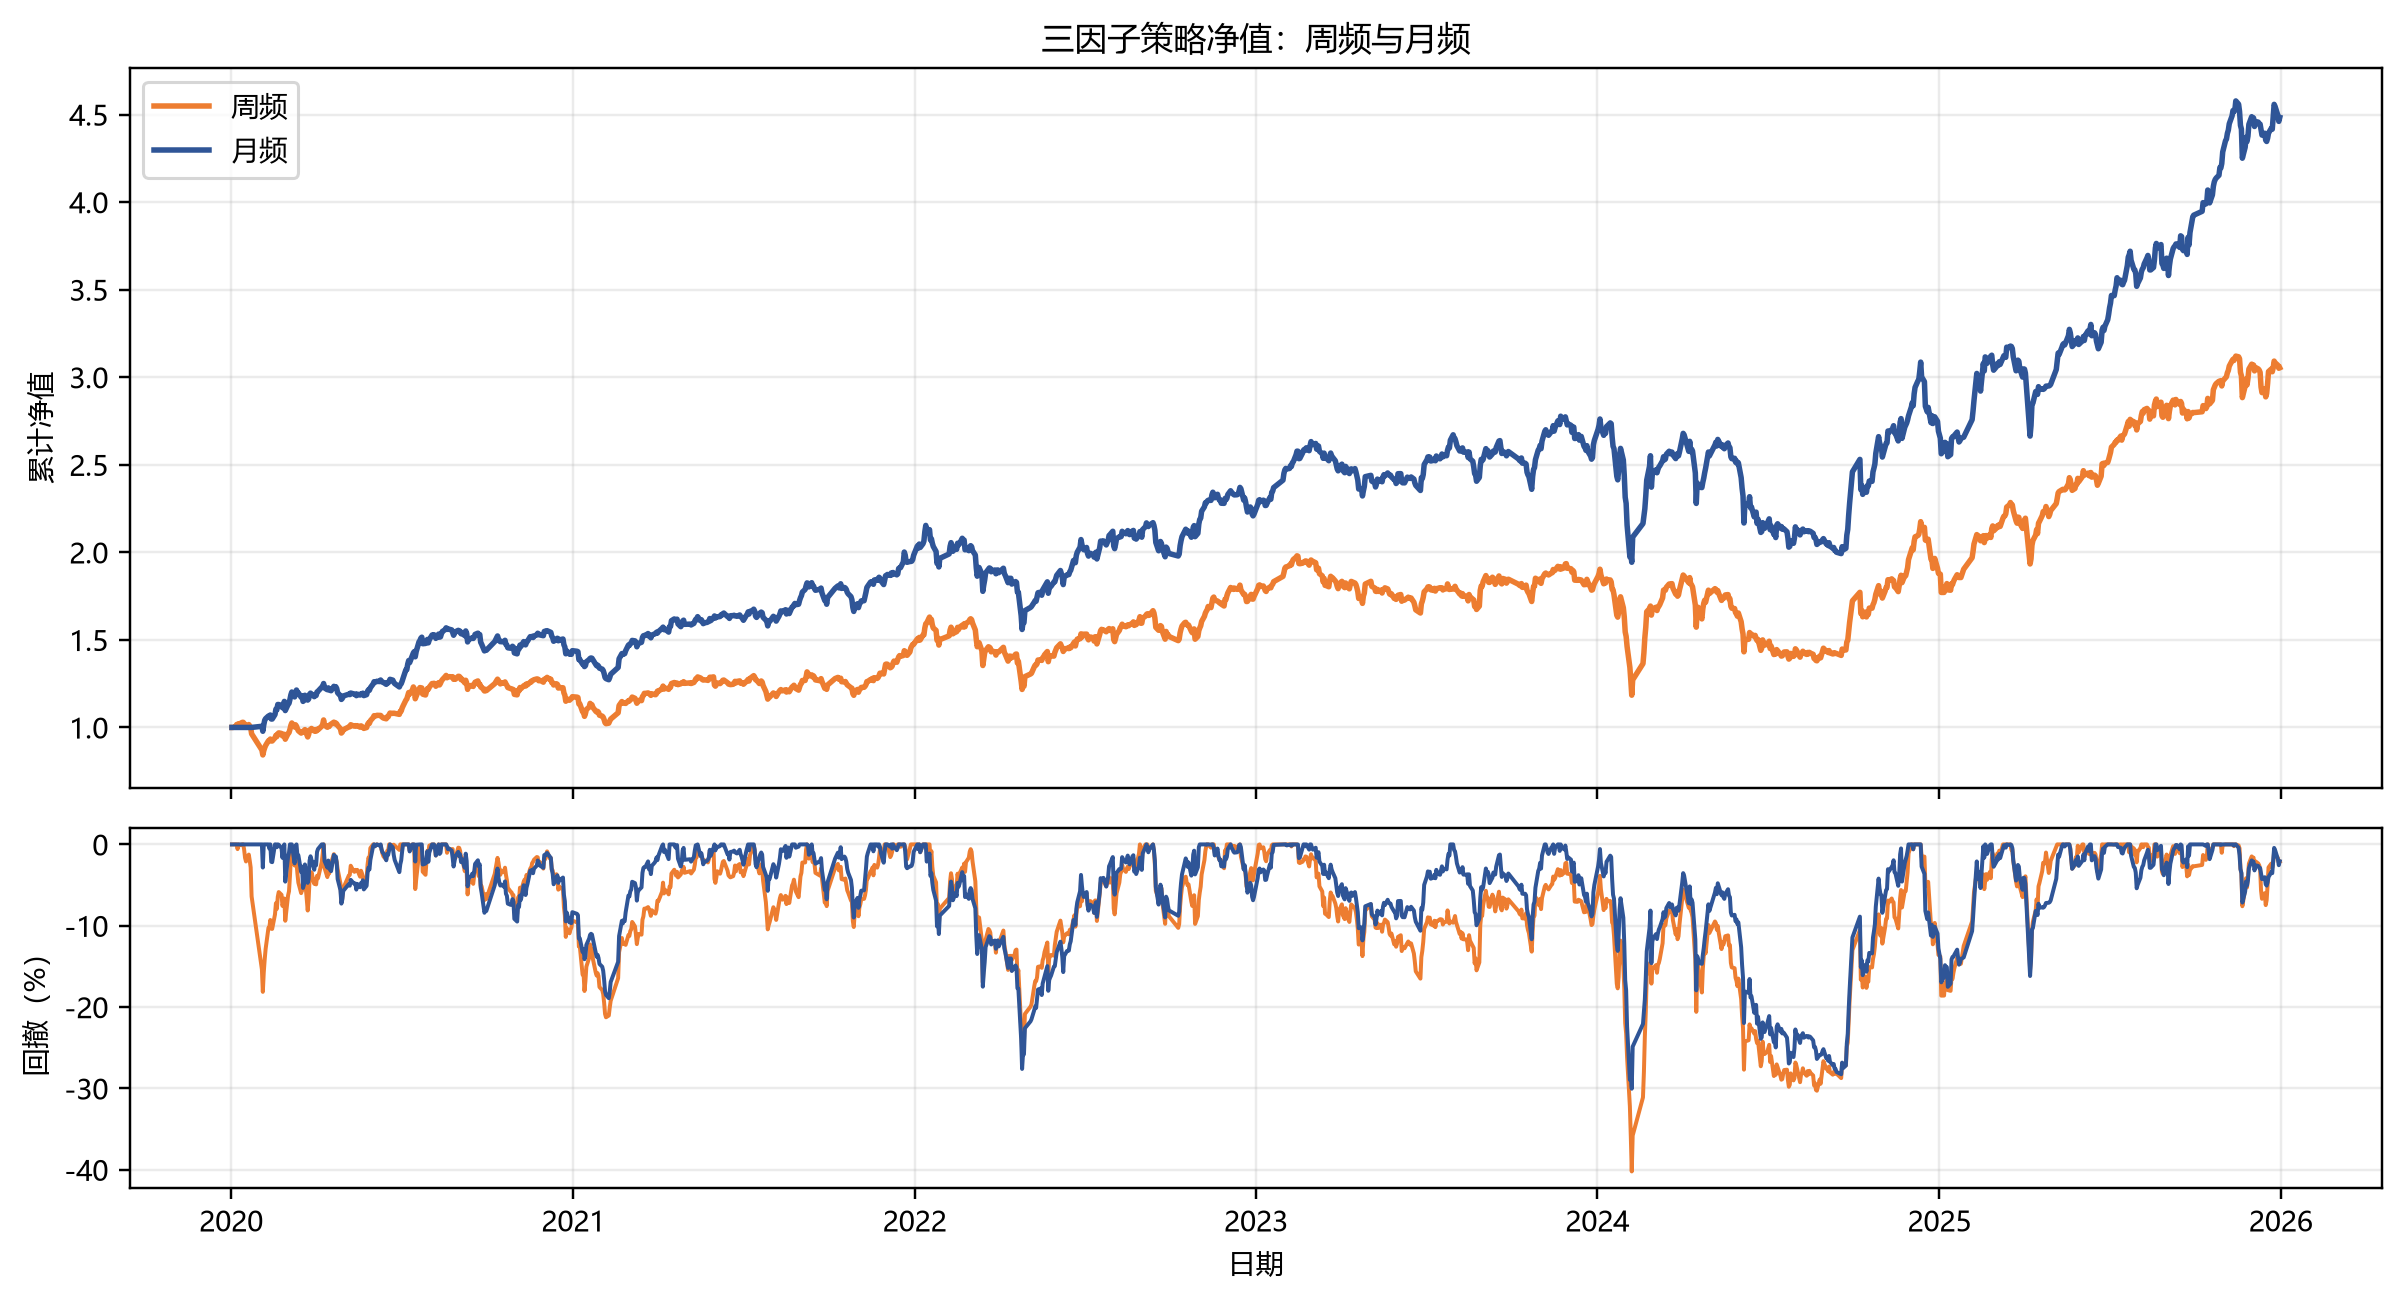
\includegraphics[width=\textwidth]{figures/03_nav_and_drawdown.png}
\caption{周频与月频三因子策略的净值和回撤}
\end{figure}

\begin{table}[H]\centering\small
\caption{周频与月频对照结果}
\begin{tabular}{lrr}
\toprule 指标 & 周频 & 月频\\\midrule
累计收益 & 205.38\% & 348.34\%\\
年化收益 & 20.40\% & 28.34\%\\
年化波动率 & 23.93\% & 22.71\%\\
Sharpe & 0.897 & 1.214\\
最大回撤 & 40.21\% & 30.04\%\\
总换手 & 517.51 & 130.55\\
显式交易成本 & 691,116元 & 233,288元\\
交易次数 & 11,304 & 2,707\\\bottomrule
\end{tabular}
\end{table}

\subsection{同成交路径的成本归因}
沿用净回测实际成交日期、价格和数量，仅把累计已付费用作为未投资现金加回，不重新成交。周频毛累计收益274.49\%、净收益205.38\%，成本拖累69.11个百分点；月频毛收益371.67\%、净收益348.34\%，拖累23.33个百分点。月频优势与较低换手和成本一致，但频率也改变持仓路径，因此不能把全部收益差异归因于费用。月频并非每年均胜出，结论属于描述性对照。

\section{拓展实验}
所有拓展均在基础三因子策略和周频/月频对照完成后单列，不改变基础任务的研究结论。

\subsection{拓展一：波动率目标}
固定月频三因子Top 20股票集合，比较等权与10\%/15\%/20\%波动率目标。风险估计只使用形成日及以前60个交易日，至少40个有效观测。波动率目标股票仓位为
\[
E_t=\min\left(1,\frac{\sigma^*}{\widehat\sigma_{t-1}}\right),
\]
不使用杠杆，剩余资金作为零收益现金。

\subsection{拓展二：ERC风险平价}
使用完整协方差矩阵和轻度收缩估计风险贡献，使Top 20内部各股票的边际风险贡献更接近。该实验回答“内部风险重分配是否优于简单等权”，与总仓位波动率控制分开解释。

\subsection{拓展三：单股权重上限与组合方案}
在ERC上加入8\%目标权重上限，并进一步与15\%波动率目标组合。8\%是调仓时目标而非每日实际权重保证；价格变化或交易受限可能造成事后超限。

\begin{figure}[H]\centering
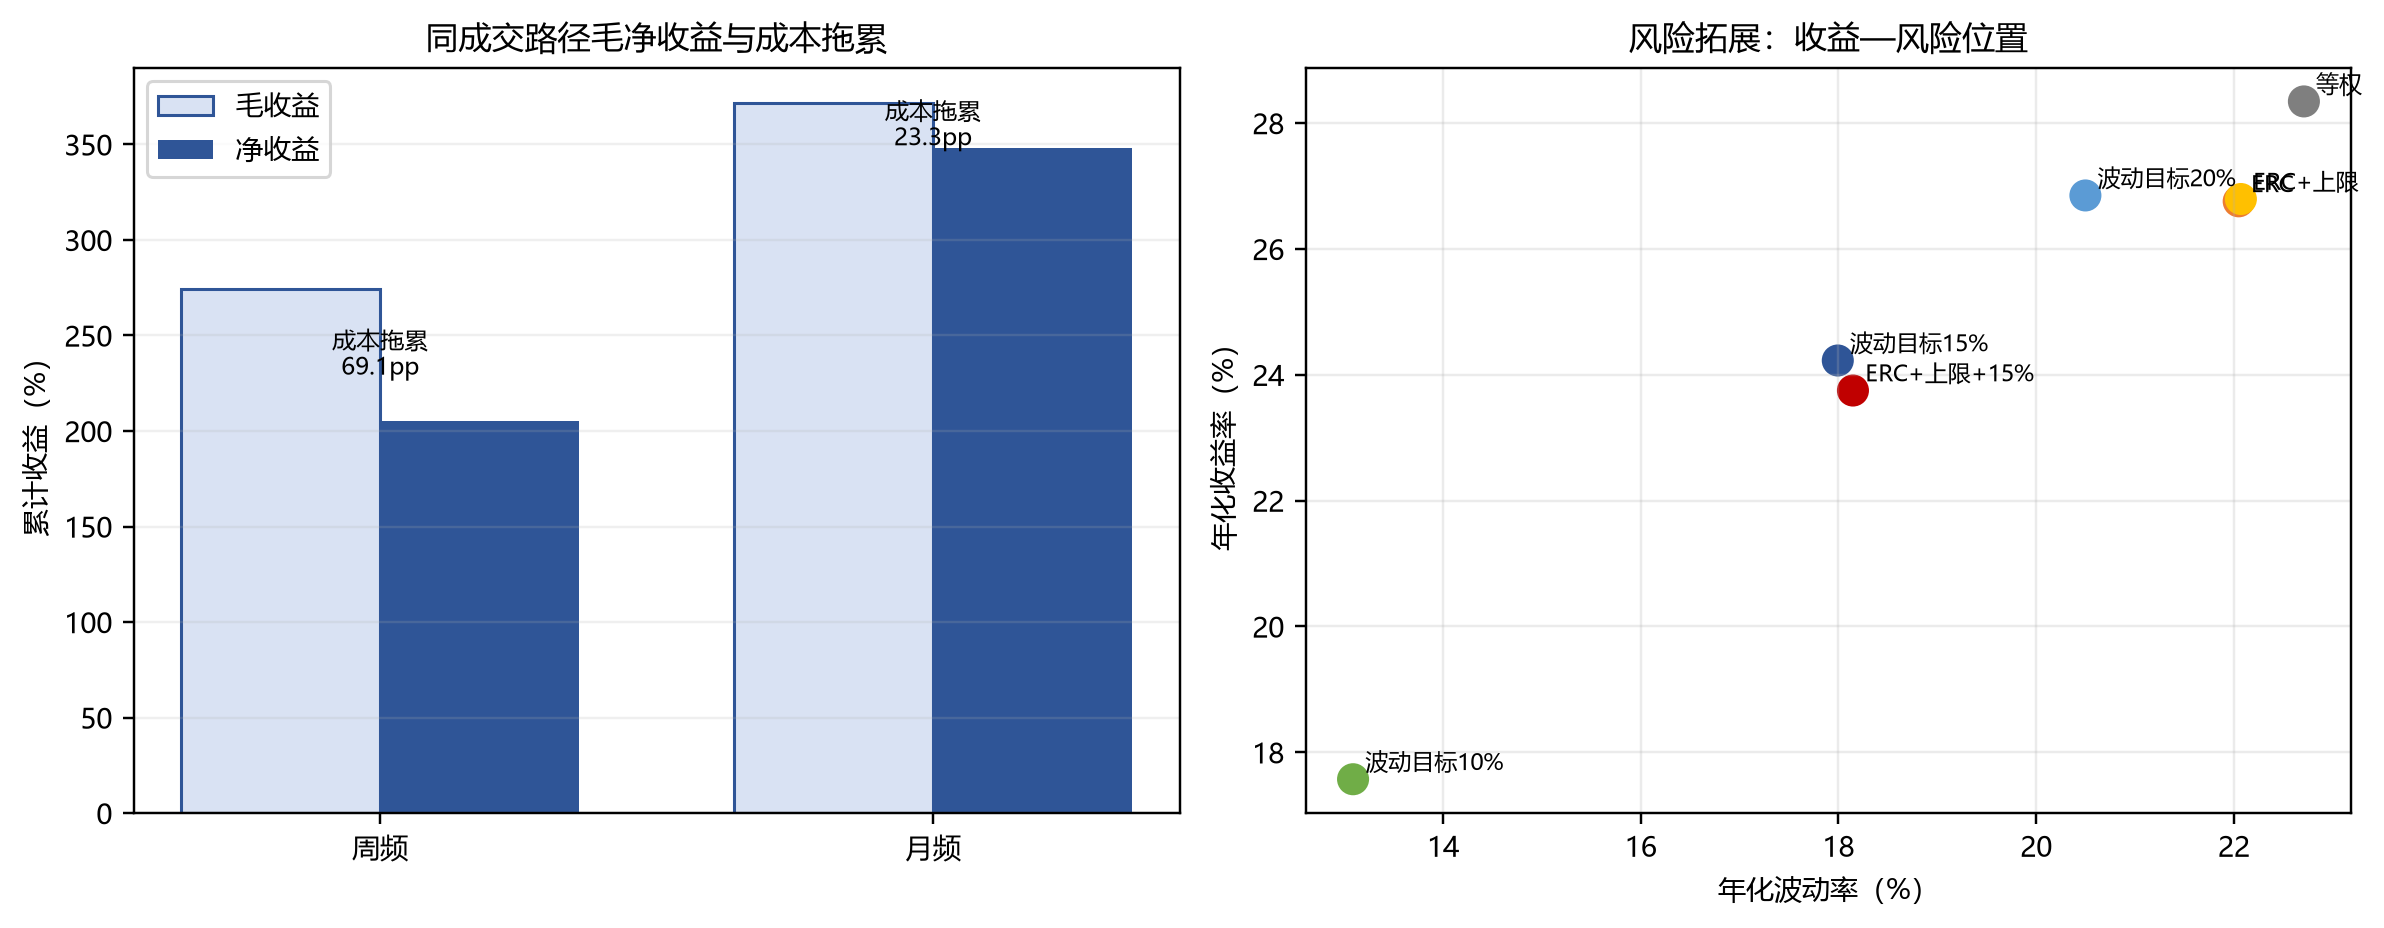
\includegraphics[width=\textwidth]{figures/04_cost_and_extension.png}
\caption{显式成本拖累与风险拓展的收益--风险比较}
\end{figure}

\begin{table}[H]\centering\footnotesize
\caption{组合与风险拓展结果}
\begin{tabular}{lrrrrr}
\toprule 方案 & 年化收益 & 年化波动 & Sharpe & 最大回撤 & 成本（元）\\\midrule
月频等权 & 28.34\% & 22.71\% & 1.214 & 30.04\% & 233,288\\
10\%波动率目标 & 17.57\% & 13.09\% & 1.303 & 18.09\% & 109,377\\
15\%波动率目标 & 24.23\% & 17.99\% & 1.296 & 25.21\% & 176,264\\
20\%波动率目标 & 26.85\% & 20.50\% & 1.264 & 28.23\% & 208,193\\
ERC风险平价 & 26.76\% & 22.05\% & 1.187 & 28.06\% & 227,592\\
ERC+8\%上限 & 26.79\% & 22.07\% & 1.187 & 28.06\% & 227,341\\
ERC+上限+15\%目标 & 23.75\% & 18.15\% & 1.266 & 24.28\% & 179,292\\\bottomrule
\end{tabular}
\end{table}

拓展结果分点解释如下：
\begin{itemize}
\item \textbf{波动率目标：}10\%目标获得最高Sharpe和最低回撤，但平均现金比例38.74\%，收益牺牲较大；15\%目标平均现金约17.06\%，在收益保留和风险下降之间更均衡。
\item \textbf{ERC风险平价：}没有改善Sharpe，说明本样本的风险改善主要来自降低总体股票暴露，而非Top 20内部重分配。
\item \textbf{权重上限：}8\%上限对结果影响有限，说明基础Top 20组合本身并未形成严重的目标权重集中。
\end{itemize}

\subsection{拓展四：动态沪深300与机器学习}
\paragraph{时点数据、因子与训练设计。}
模型拓展使用73个月历史成分权重快照，涉及398只历史成分股；成分从生效日向后使用，财务指标按公告日做as-of连接。10个输入因子覆盖量价、价值和质量，每个信号日依次缩尾、行业与市值中性化并标准化。训练严格按时间推进：2020--2022为初始训练，2023--2024用于参数和组合规则选择，2025仅作一次冻结样本外测试。每月扩展窗口重新训练，但只有未来20日标签已完整退出的样本可以进入训练。

Ridge提供线性基准，LightGBM学习非线性与交互关系。验证期最优LightGBM参数的Rank IC为0.0486，而Ridge约为$-0.0042$。Qlib 0.9.7作为因子研究接口，首批透明复算21个Alpha158 OHLCV表达式；2025月度Rank IC较高者包括RSV20（0.079）、RSV5（0.063）和WVMA20（0.039）。这些结果只作为下一轮候选，不回填已经冻结的2025策略。

\paragraph{逐日执行与状态切换。}
月末收盘形成目标，下一交易日开盘成交；开盘涨停不买、跌停不卖，停牌或零成交阻断订单，现金和残留持仓逐日对账。验证期选定126日相对强弱状态规则，每月只切换一次：弱状态持有沪深300，强状态切换到防御型LightGBM Top10，切换另按16bp保守收费。该规则在查看2025结果前冻结。

\begin{figure}[H]\centering
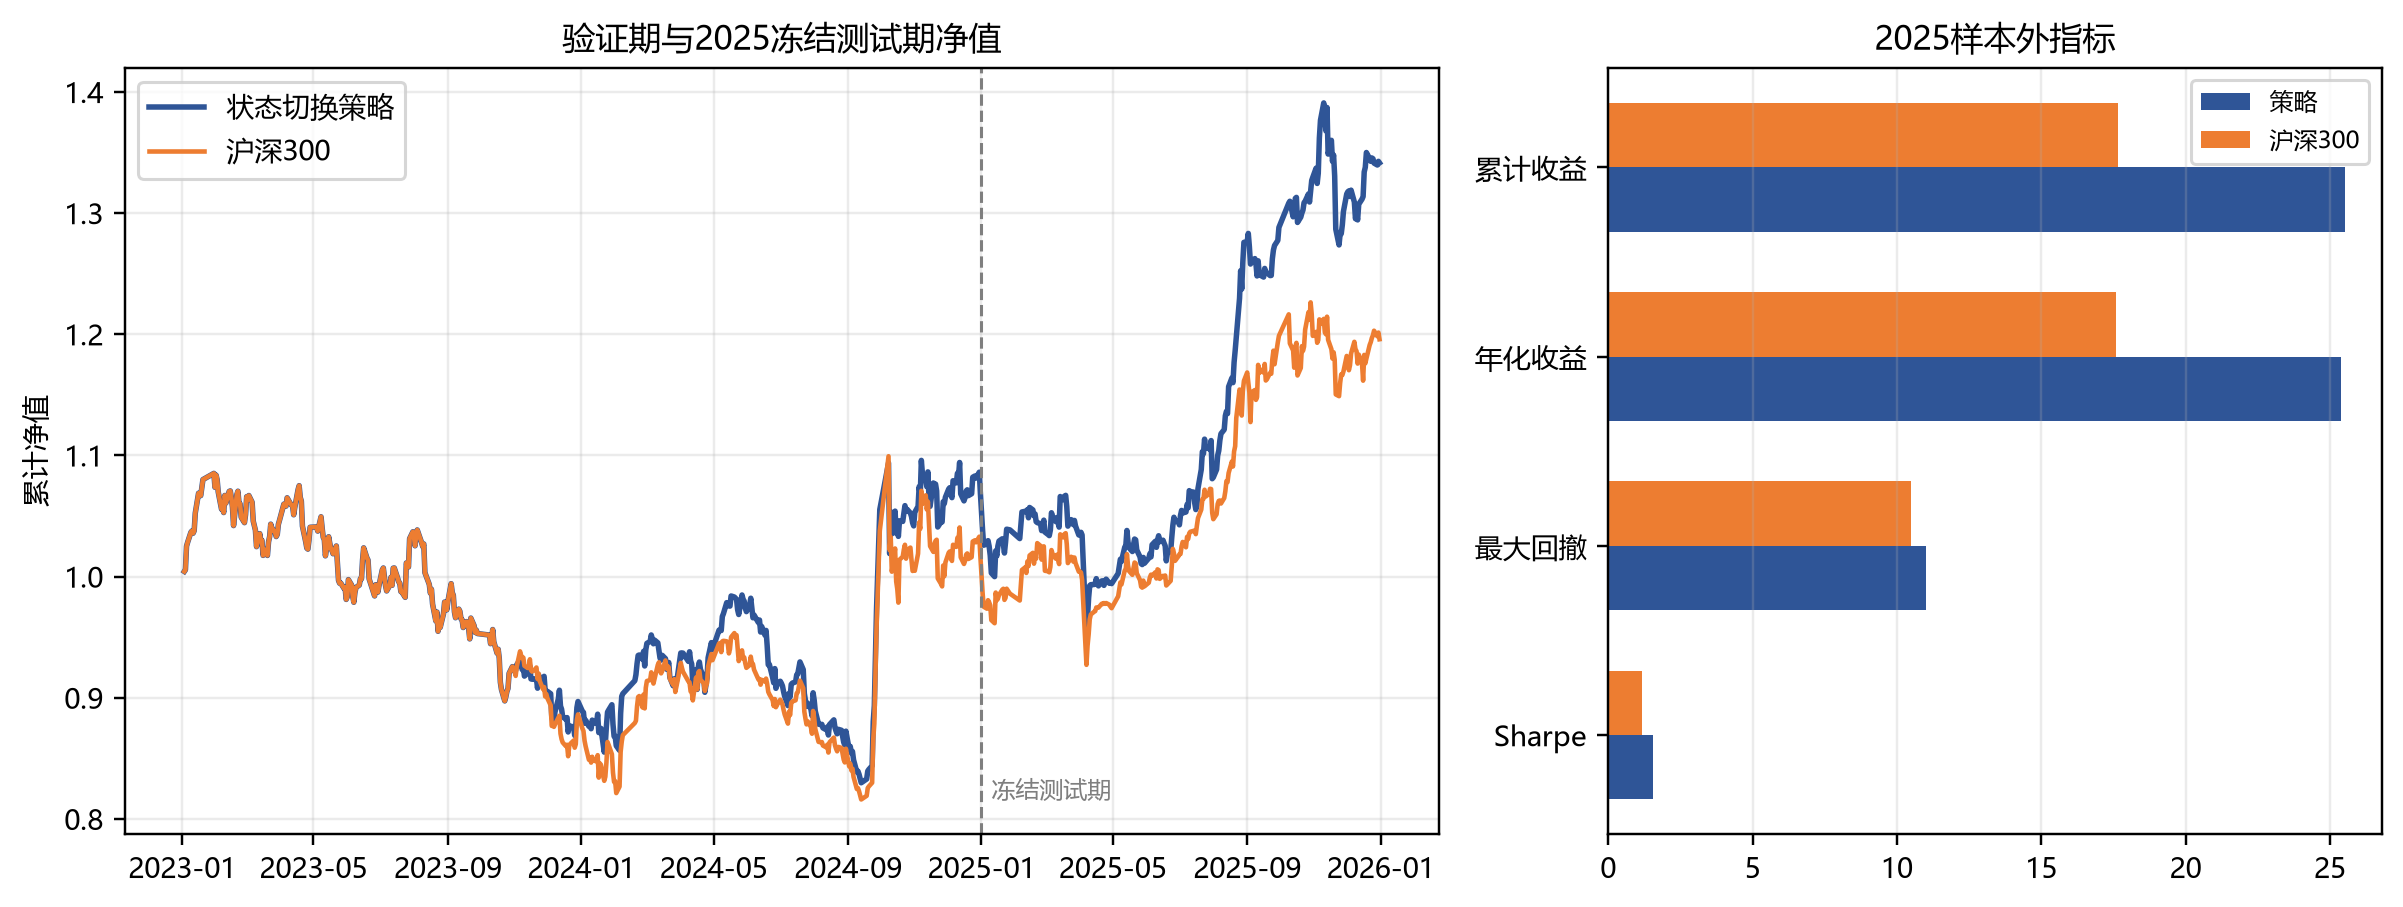
\includegraphics[width=\textwidth]{figures/05_model_extension.png}
\caption{动态沪深300状态切换策略与冻结样本外结果}
\end{figure}

\begin{table}[H]\centering\small
\caption{状态切换策略与沪深300对比}
\begin{tabular}{llrrrr}
\toprule 期间 & 策略 & 累计收益 & 年化收益 & 最大回撤 & Sharpe\\\midrule
2023--2024验证 & 状态切换 & 6.87\% & 3.38\% & 23.53\% & 0.280\\
2023--2024验证 & 沪深300 & 1.63\% & 0.81\% & 24.80\% & 0.133\\
2025冻结测试 & 状态切换 & 25.51\% & 25.40\% & 11.02\% & 1.545\\
2025冻结测试 & 沪深300 & 17.66\% & 17.58\% & 10.49\% & 1.159\\\bottomrule
\end{tabular}
\end{table}

\subsection{拓展五：Qlib因子库与研究工作台}
Qlib仅作为新因子研究接口，当前21个透明表达式的诊断结果不回填正式基础策略。网页研究工作台直接读取审计CSV，允许切换基础结果、风险拓展及模型候选，并同步显示净值、回撤和指标；网页不重新计算绩效。同花顺部分仅导出待人工复核的模拟订单清单，不自动登录或下单。

\section{结论、局限与复现}
\subsection{主要结论}
主线结论只有两点：其一，低波动、短期反转和流动性三个维度形成逻辑互补的基础信号；其二，在其他条件一致时，月频相较周频具有更低换手、成本和回撤。拓展实验另行表明15\%波动率目标能在收益保留与风险下降间取得平衡；ERC和权重上限没有改善Sharpe。动态沪深300机器学习结果属于附加探索，不作为基础三因子策略成立的必要条件。

\subsection{局限与下一步}
基础回测未建模冲击成本、滑点和100股整手约束，现金收益设为0，历史ST依赖名称区间，退市残余持仓按零回收。模型拓展虽已做行业与市值中性化和逐日开盘撮合，但仍缺少冲击成本、整手约束与真实模拟账户成交验证。传统t统计量未修正重叠标签、自相关和多重搜索。下一步将Qlib候选因子放入新的扩展窗口，并以新增2026数据建立新的最终留出期，而不是继续利用2025调参。

\subsection{复现信息}
项目提供测试、下载、清洗、资产池、因子、诊断、回测、模型拓展、网页和最终复现包入口。原始数据共有9,503个文件并逐项记录SHA-256；另提供10只股票、57个交易日的离线小样本。最终清单记录源码、配置、文档、证据输出和DuckDB引用，并在元数据中写入Git提交及生成前工作区状态。

\begin{table}[H]\centering\small
\caption{主要复现入口}
\begin{tabularx}{\textwidth}{lX}
\toprule 模块 & 入口\\\midrule
因子构建 & \code{scripts/05\_factors/05\_run\_factor\_pipeline.py}\\
因子诊断 & \code{scripts/06\_evaluation/06\_run\_evaluation\_pipeline.py}\\
基础回测 & \code{scripts/07\_backtest/06\_run\_backtest\_pipeline.py}\\
对照实验 & \code{scripts/08\_experiments/04\_run\_weekly\_vs\_monthly\_experiment.py}\\
风险拓展 & \code{scripts/09\_extensions/04\_run\_portfolio\_risk\_extension.py}\\
模型拓展 & \code{scripts/08\_experiments/10\_run\_regime\_overlay.py}\\
Qlib诊断 & \code{scripts/08\_experiments/12\_run\_qlib\_alpha158\_subset.py}\\
最终复现包 & \code{scripts/10\_reproducibility/04\_run\_final\_reproduction\_package.py}\\\bottomrule
\end{tabularx}
\end{table}

\subsection{课程要求与验收证据索引}
为避免仅声明“已经完成”，表\ref{tab:requirement-map}将课程要求直接对应到可核验的报告证据与复现产物。
\begin{table}[H]\centering\footnotesize
\caption{课程要求--报告证据对照}\label{tab:requirement-map}
\begin{tabularx}{\textwidth}{p{3.1cm}Xp{3.4cm}}
\toprule 课程要求 & 本报告中的直接证据 & 可复现产物\\\midrule
数据接入、清洗与质量报告 & 第2节的数据规模、互斥清洗对账、唯一键与异常处理 & 原始/清洗表、质量报告、SHA-256清单\\
三个逻辑不同的因子及诊断 & 第3--4节因子卡、统一方向、IC、Rank IC与五分组 & 因子长表、诊断CSV和图片\\
可配置回测与绩效分析 & 第5节信号时点、持仓、费用、成交限制与一致性检查 & YAML配置、交易日志、净值与指标表\\
小型对照实验 & 第6节周频与月频仅改变调仓频率的对照 & 两组同口径配置和检查输出\\
自主拓展 & 第7节分点列出的波动率目标、ERC、权重上限、模型与工作台 & 风险拓展、模型审计、Qlib诊断和网页\\
复现包与研究报告 & 第8节入口、环境、快照、小样本及校验值 & README、一键入口、清单和离线小样本\\
\bottomrule
\end{tabularx}
\end{table}

\end{document}
